\clearpage
\chapter{Neutron calibration with a californium source}

%https://arxiv.org/pdf/0811.0735.pdf
%https://www.sno.phy.queensu.ca/sno/papers/labranche_phd.pdf
%https://www.sno.phy.queensu.ca/sno/papers/lyon_phd.pdf

To measure neutron tagging efficiency, an americium-beryllium (Am-Be) source is placed inside
a bismuth germanite (BGO) crystal scintillator and the whole device is usually deployed %
at the centre of the water Cherenkov detector.
The americium-241 goes through $\alpha$ decay with a half-life of 432.6\,y. [100\% ?]
The $\alpha$ particle is captured by the \tapi{9}Be nuclei to become \tapi{12}C\tapi{*} with the emission of a neutron.
The carbon de-excites to the ground state with sometimes the emission of a 4.43\,MeV photon.
The gamma ray is promptly captured by the BGO crystal, and the scintillation light triggers the detector.
The neutron thermalises in the water with an average time of roughly 200\,\textmu s, %
before begin captured on a hydrogen nucleus with the release of a 2.2\,MeV photon.
Neutron tagging efficiency on hydrogen in SK was measured to be $(19.0\pm0.2)$\,\%, %
using a unbinned maximum likelihood fitting~\cite{}.
Neutrons released by beryllium have an energy ranging from 2-10 MeV, %
much less than the average neutron energy following atmospheric neutrino interactions.
Thus, we can make the assumption that the location of the Am-Be apparatus is roughly the same %
as the neutron capture vertex.


Another possible source for neutron calibration is californium-252, which %
undergoes $\alpha$-emissions (96.91\%) and spontaneous fission (SF) (3.09\%).
With a half-life of 2.645\,y, a \tapi{252}Cf source has a higher activity compared to an Am-Be source %
with the same number of nucleons.
Furthermore, the SF process emits an average of 3.75 neutrons per fission and an average of 10.3 photons %
having a total energy of 8.2\,Mev.
As for the case of Am-Be, the photons can be collected by a scintillating material to tag the %
emission of neutrons.
After this trigger signal, multiple neutron captures on hydrogen are expected, %
separated by short intervals in time.
The yield of multiple neutrons is another advantage of \tapi{252}Cf that %
the SNO collaboration exploited to develop a method, called \emph{Time Series Analysis} method that uses %
multiplicity and time intervals between the detected events %
to find the neutron detection efficiency, the neutron mean life inside the detector, %
and activity from non-fission events.
The fast-neutron and photon energy spectra are shown in \ref{fig:spectra}: %
the neutrons are emitted with a most-probable energy of 0.7\,MeV and an average energy of 2.1\,MeV.

\begin{figure}
	\begin{minipage}[t]{0.45\textwidth}
		\centering
		\resizebox{\textwidth}{!}{\input{spectrum.tex}}
		\caption{Normalised energy distribution of neutron and photons emitted %
			by SF events of a \tapi{252}Cf source~\cite{PhysRev.104.699, PhysRev.108.411}.}
		\label{fig:spectra}
	\end{minipage}
	\hfill
	\begin{minipage}[t]{0.56\textwidth}
		\centering
		\includegraphics[width=0.4\linewidth]{device.png}
		\raisebox{2.5em}{\includegraphics[width=0.4\linewidth]{device_in.png}}
		\captionof{figure}{Setup used to test the californium source.}
		\label{fig:setup}
	\end{minipage}
\end{figure}


A \tapi{252}Cf source was purchased by QMUL with an activity of 4.3\,kBq, measured on the 28\tapi{th} of July, 2017.
The californium is encapsulated in a double hull stainless steel cylinder, 9.5\,mm in diameter and 37.5\,mm high.
The source is tested in a simple calibration device (see Fig.~\ref{fig:setup}), which consists of a cylindrical plastic scintillator %
(EJ-200), coated with mylar to contain optical photons, and optically coupled to a ET Enterprise 9902B series~PMT.
A hole, coaxial to the plastic cylinder, allows to place the source in the middle of the scintillator.
The cylinder is 3\,in in length and 1.5\,in in diameter.
With this setup, the rate of photons emitted by the \tapi{252}Cf source can be measured; %
we used a Struck SIS3316 14-bit VME digitiser to count the number of photon triggers from the PMT and %
a daisy-chain of NIM amplifier, threshold, and discriminator is used before the digitiser to optimise the signal.
Without the source inside the scintillator, an event rate of 1.633\,Hz was measured, whereas with the source inside %
the rate increases to 41.395\,Hz.
The distributions of the PMT peaks collected by the digitiser are shown in Fig.~\ref{fig:source}.
A predicted activity of 3.1\,kBq is expected on the day when the measurement was %
taken---446 days after the activity measurement---which translates to a SF rate of 96.46\,Hz.
The SF tagging efficiency with this setup is therefore around~41\,\%.

\begin{figure}
	\begin{minipage}[t]{0.48\textwidth}
		\centering
		\resizebox{\textwidth}{!}{\input{peaksources.tex}}
		\captionof{figure}{Distribution of PMT peaks measured with source inside (black) and source removed from the scintillator~(red).}
		\label{fig:source}
	\end{minipage}
	\hfill
	\begin{minipage}[t]{0.48\textwidth}
		\centering
		\resizebox{\textwidth}{!}{\input{QE.tex}}
		\captionof{figure}{Plot showing PMT quantum efficiency (red), the scintillator yield (blue), %
			their convolution (magenta) and the distributions of photon collected by the PMT in the GEANT4 simulation of optical photons (black).}
		\label{fig:QE}
	\end{minipage}
\end{figure}

We performed a GEANT4 simulation of the setup, with the aim of optimising the calibration device.
An ideal calibration device would absorb all the photons converting them into visible light without affect the neutrons.
The plot in Fig.~\ref{fig:QE} shows the correct implementation of the scintillator and PMT efficiencies, %
as there is good agreement with the MC distribution and the expected optical photon spectrum.
The scintillating volume is therefore varied in the simulation to study the preformance of the decive.
Bismuth germanate oxide (BGO) crystal and a generic vinyltouluene plastic are studied as scintillating materials.
The size of the scintillator is also varied and shapes of a cube and a cylinder with equal diameter and height are tested.
The simulation keeps track of the energy deposited in the scintillator and the number of neutrons escaping the device.
The result is shown in Fig.~\ref{fig:geant4}.
Unsurprisingly, the BGO crystal performs better than the plastic scintillator, %
with the optimal volume being a cube with 12\,cm sides.
The hydrogen in the plastic thermalises neutrons, which can have an impact on the thermalisation time %
in a water Cherenkov detector.

\begin{figure}
	\centering
	\resizebox{0.9\textwidth}{!}{% GNUPLOT: LaTeX picture with Postscript
\begingroup
  \makeatletter
  \providecommand\color[2][]{%
    \GenericError{(gnuplot) \space\space\space\@spaces}{%
      Package color not loaded in conjunction with
      terminal option `colourtext'%
    }{See the gnuplot documentation for explanation.%
    }{Either use 'blacktext' in gnuplot or load the package
      color.sty in LaTeX.}%
    \renewcommand\color[2][]{}%
  }%
  \providecommand\includegraphics[2][]{%
    \GenericError{(gnuplot) \space\space\space\@spaces}{%
      Package graphicx or graphics not loaded%
    }{See the gnuplot documentation for explanation.%
    }{The gnuplot epslatex terminal needs graphicx.sty or graphics.sty.}%
    \renewcommand\includegraphics[2][]{}%
  }%
  \providecommand\rotatebox[2]{#2}%
  \@ifundefined{ifGPcolor}{%
    \newif\ifGPcolor
    \GPcolortrue
  }{}%
  \@ifundefined{ifGPblacktext}{%
    \newif\ifGPblacktext
    \GPblacktexttrue
  }{}%
  % define a \g@addto@macro without @ in the name:
  \let\gplgaddtomacro\g@addto@macro
  % define empty templates for all commands taking text:
  \gdef\gplbacktext{}%
  \gdef\gplfronttext{}%
  \makeatother
  \ifGPblacktext
    % no textcolor at all
    \def\colorrgb#1{}%
    \def\colorgray#1{}%
  \else
    % gray or color?
    \ifGPcolor
      \def\colorrgb#1{\color[rgb]{#1}}%
      \def\colorgray#1{\color[gray]{#1}}%
      \expandafter\def\csname LTw\endcsname{\color{white}}%
      \expandafter\def\csname LTb\endcsname{\color{black}}%
      \expandafter\def\csname LTa\endcsname{\color{black}}%
      \expandafter\def\csname LT0\endcsname{\color[rgb]{1,0,0}}%
      \expandafter\def\csname LT1\endcsname{\color[rgb]{0,1,0}}%
      \expandafter\def\csname LT2\endcsname{\color[rgb]{0,0,1}}%
      \expandafter\def\csname LT3\endcsname{\color[rgb]{1,0,1}}%
      \expandafter\def\csname LT4\endcsname{\color[rgb]{0,1,1}}%
      \expandafter\def\csname LT5\endcsname{\color[rgb]{1,1,0}}%
      \expandafter\def\csname LT6\endcsname{\color[rgb]{0,0,0}}%
      \expandafter\def\csname LT7\endcsname{\color[rgb]{1,0.3,0}}%
      \expandafter\def\csname LT8\endcsname{\color[rgb]{0.5,0.5,0.5}}%
    \else
      % gray
      \def\colorrgb#1{\color{black}}%
      \def\colorgray#1{\color[gray]{#1}}%
      \expandafter\def\csname LTw\endcsname{\color{white}}%
      \expandafter\def\csname LTb\endcsname{\color{black}}%
      \expandafter\def\csname LTa\endcsname{\color{black}}%
      \expandafter\def\csname LT0\endcsname{\color{black}}%
      \expandafter\def\csname LT1\endcsname{\color{black}}%
      \expandafter\def\csname LT2\endcsname{\color{black}}%
      \expandafter\def\csname LT3\endcsname{\color{black}}%
      \expandafter\def\csname LT4\endcsname{\color{black}}%
      \expandafter\def\csname LT5\endcsname{\color{black}}%
      \expandafter\def\csname LT6\endcsname{\color{black}}%
      \expandafter\def\csname LT7\endcsname{\color{black}}%
      \expandafter\def\csname LT8\endcsname{\color{black}}%
    \fi
  \fi
    \setlength{\unitlength}{0.0500bp}%
    \ifx\gptboxheight\undefined%
      \newlength{\gptboxheight}%
      \newlength{\gptboxwidth}%
      \newsavebox{\gptboxtext}%
    \fi%
    \setlength{\fboxrule}{0.5pt}%
    \setlength{\fboxsep}{1pt}%
\begin{picture}(14400.00,7632.00)%
    \gplgaddtomacro\gplbacktext{%
      \csname LTb\endcsname%%
      \put(444,440){\makebox(0,0)[r]{\strut{}$0$}}%
      \put(444,1789){\makebox(0,0)[r]{\strut{}$0.2$}}%
      \put(444,3138){\makebox(0,0)[r]{\strut{}$0.4$}}%
      \put(444,4486){\makebox(0,0)[r]{\strut{}$0.6$}}%
      \put(444,5835){\makebox(0,0)[r]{\strut{}$0.8$}}%
      \put(444,7184){\makebox(0,0)[r]{\strut{}$1$}}%
      \put(576,220){\makebox(0,0){\strut{}$0$}}%
      \put(2304,220){\makebox(0,0){\strut{}$10$}}%
      \put(4032,220){\makebox(0,0){\strut{}$20$}}%
      \put(5759,220){\makebox(0,0){\strut{}$30$}}%
      \put(4032,3812){\makebox(0,0)[l]{\strut{}BGO scintillator}}%
    }%
    \gplgaddtomacro\gplfronttext{%
      \csname LTb\endcsname%%
      \put(-172,3980){\rotatebox{-270}{\makebox(0,0){\strut{}Percentage (\%)}}}%
      \put(4031,-110){\makebox(0,0){\strut{}Size (cm)}}%
      \csname LTb\endcsname%%
      \put(6896,1273){\makebox(0,0)[r]{\strut{}Gamma aborsbed energy (\%)}}%
      \csname LTb\endcsname%%
      \put(6896,1053){\makebox(0,0)[r]{\strut{}Neutron surviving (\%)}}%
      \csname LTb\endcsname%%
      \put(6896,833){\makebox(0,0)[r]{\strut{}Cube}}%
      \csname LTb\endcsname%%
      \put(6896,613){\makebox(0,0)[r]{\strut{}Cylinder}}%
    }%
    \gplgaddtomacro\gplbacktext{%
      \csname LTb\endcsname%%
      \put(7356,440){\makebox(0,0)[r]{\strut{}}}%
      \put(7356,1789){\makebox(0,0)[r]{\strut{}}}%
      \put(7356,3138){\makebox(0,0)[r]{\strut{}}}%
      \put(7356,4486){\makebox(0,0)[r]{\strut{}}}%
      \put(7356,5835){\makebox(0,0)[r]{\strut{}}}%
      \put(7356,7184){\makebox(0,0)[r]{\strut{}}}%
      \put(14399,220){\makebox(0,0){\strut{}$40$}}%
      \put(7488,220){\makebox(0,0){\strut{}$0$}}%
      \put(9216,220){\makebox(0,0){\strut{}$10$}}%
      \put(10944,220){\makebox(0,0){\strut{}$20$}}%
      \put(12671,220){\makebox(0,0){\strut{}$30$}}%
      \put(10944,3812){\makebox(0,0)[l]{\strut{}Plastic scintillator}}%
    }%
    \gplgaddtomacro\gplfronttext{%
      \csname LTb\endcsname%%
      \put(10943,-110){\makebox(0,0){\strut{}Size (cm)}}%
      \csname LTb\endcsname%%
      \put(13808,7348){\makebox(0,0)[r]{\strut{}Gamma aborsbed energy (\%)}}%
      \csname LTb\endcsname%%
      \put(13808,7128){\makebox(0,0)[r]{\strut{}Neutron surviving (\%)}}%
      \csname LTb\endcsname%%
      \put(13808,6908){\makebox(0,0)[r]{\strut{}Cube}}%
      \csname LTb\endcsname%%
      \put(13808,6688){\makebox(0,0)[r]{\strut{}Cylinder}}%
    }%
    \gplbacktext
    \put(0,0){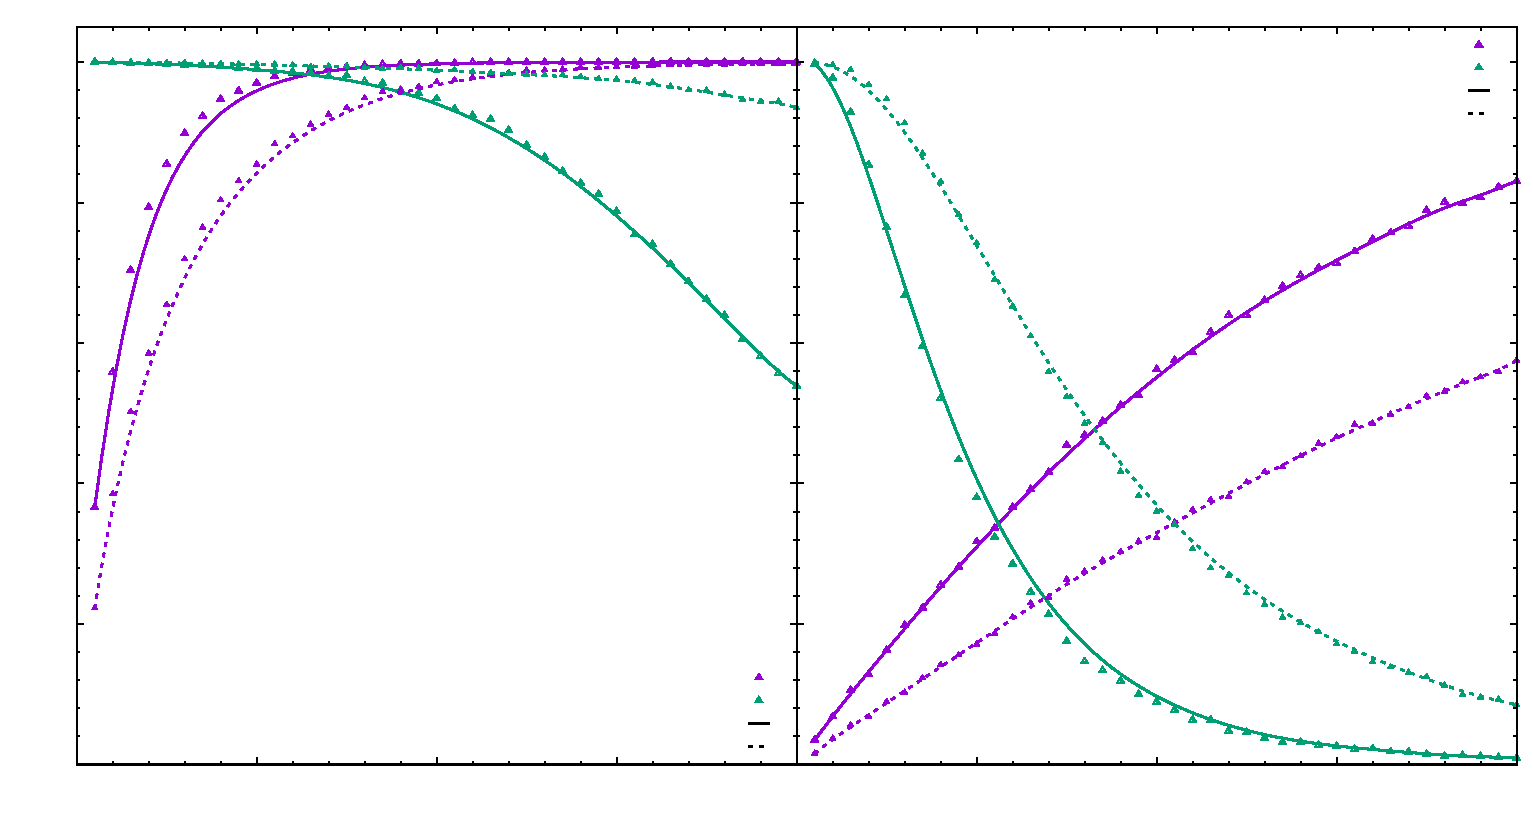
\includegraphics{pics/n_vs_gamma}}%
    \gplfronttext
  \end{picture}%
\endgroup
}
	\caption{Result of the GEANT4 simulation, showing the performance of different scintillators.
		Two shapes are tested: a cube (solid lines) and a cylinder with equal diameter and hie hgt (dashed lines).
		The percentage of energy absorbed by the scintillator (purple) and the percentage of neutrons escaping the %
		scintillators (green) are estimated for every simulation.
		Left: BGO is used as scintillating material. Right: a generic vinyltouluene plastic is used.}
	\label{fig:geant4}
\end{figure}


%To verify neutron tagging efficiency given above, experimental tests were conducted with an Am/Be source embedded in a bismuth germanite (BGO) scintillator. The prompt and delayed event-pair is generated via: α + 9Be →12
%C∗+n; 12C∗ →12 C+γ(prompt); n+p → d+γ(delayed).
%The scintillation light induced by 4.43 MeV deexcitation γ
%serves as the primary event. Note that the reaction to the
%ground state of 12C also exists, where no 4.43 MeV deexcitation γ is emitted. The experimental apparatus was
%deployed at the center of the tank, during which the trigger
%gate to catch 2.2 MeV γ was temporarily enlarged to 800
%μs in order to obtain a complete neutron capture time spectrum. To estimate source related background (e.g. ground
%transition neutron), 10 Hz 800μs random trigger data was
%also taken.
%The final N10 distribution after all cuts applied is shown in
%Fig. 2, where for Am/Be data all backgrounds are subtracted according to random trigger data. Signal efficiencies for
%MC and data are (19.2±0.1)% and (19.0±0.2)%, respectively. Data is in good agreement with MC. Fig. 3 shows
%the distribution of time difference (ΔT) between delayed
%neutron signal and prompt event. The neutron lifetime in
%pure water is measured to be (201.8 ± 4.7)μs using a unbinned maximum likelihood fitting as shown in Fig. 3.
%
%The Am-Be source is embedded in a 5 cm cube of BGO scintillator (see figure 8.27)
%to amplify the light released by the 4.4 MeV γ-ray, such that it will activate the SHE
%trigger in the detector. Upon triggering SHE stores 35µs of data, and then an extended
%AFT trigger is activated to store an additional 800µs, and grant a more complete view
%the neutron capture time spectrum.
%Figure 8.27: Am-Be crystal embedded in a 5 cm cube of BGO scintillator. This is
%held in an acrylic case.
%This configuration was set up in 3 different locations around the tank: the centre (35.3,
%-70.7, 0) cm (Centre), near the side of the barrel (35.3, -1201.9, 0) cm (Y12), and near
%the top of the tank (35.3, -70.7, 1500.0) cm (Z15). Random data was also taken with
%the apparatus in the centre, using a 10Hz trigger, to study the irreducible background
%from the ground-state transition.
%
%
%Neutron tagging is then performed on the remaining Am-Be dataset, and a 2.2 MeV
%γ-ray MC. There are some differences between this study and the atmospheric neutrino study discussed up until now. Neutrons released by Beryllium have an energy
%ranging from 2-10 MeV, much less than the average neutron energy following atmospheric neutrino interactions. Thus, we can make the assumption that the location of
%the Am-Be apparatus is roughly the same as the neutron capture vertex. This raises
%the expected neutron detection efficiency in accordance with figure 8.23. In addition,
%Chapter 8. Neutron Tagging 140
%the PMT after-pulse observed following high energy atmospheric neutrino events (figure 8.5) is not produced to the same extent after Am-Be events, so neutron searching
%is started at 5µs (previously > 18µs) after the primary trigger. The AFT trigger for
%Am-Be is also extended, allowing neutron-searching until 835µs after the initial trigger.
%The efficiency is calculated by fitting the timing distribution of neutron candidates to a
%constant background + exponentially decaying signal representing the neutron capture
%lifetime.
